\documentclass[11pt,twoside]{article}
\usepackage{etex}
\newcommand{\num}{6{} }

\raggedbottom

%geometry (sets margin) and other useful packages
\usepackage{geometry}
\geometry{top=1in, left=1in,right=1in,bottom=1in}
 \usepackage{graphicx,booktabs,calc}

%=== GRAPHICS PATH ===========
\graphicspath{{./images/}}
% Marginpar width
%Marginpar width
\newcommand{\pts}[1]{\marginpar{ \small\hspace{0pt} \textit{[#1]} } } 
\setlength{\marginparwidth}{.5in}
%\reversemarginpar
%\setlength{\marginparsep}{.02in}

%% Fonts
% \usepackage{fourier}
% \usepackage[T1]{pbsi}

\usepackage{lmodern}
\usepackage[T1]{fontenc}
%\usepackage{minted}

\usepackage{rotating}
%% Cite Title
\usepackage[style=authoryear,maxcitenames=2,natbib]{biblatex}
\addbibresource{../bib/references.bib}

%%% Counters
\usepackage{chngcntr,mathtools}
\counterwithout{figure}{section}
\counterwithout{table}{section}

\numberwithin{equation}{section}

%% Captions
\usepackage{caption}
\captionsetup{
  labelsep=quad,
  justification=raggedright,
  labelfont=sc
}

%AMS-TeX packages
\usepackage{amssymb,amsmath,amsthm} 
\usepackage{bm}
\usepackage[mathscr]{eucal}
\usepackage{colortbl}
\usepackage{color}


\usepackage{epstopdf,subfigure,hyperref,enumerate,polynom,polynomial}
\usepackage{multirow,minitoc,fancybox,array,multicol}

\definecolor{slblue}{rgb}{0,.3,.62}%
%\renewcommand{\chaptermark}[1]{ \markboth{#1}{} }
\renewcommand{\sectionmark}[1]{ \markright{#1}{} }

\usepackage{fancyhdr}
\pagestyle{fancy}
%\addtolength{\headwidth}{\marginparsep} %these change header-rule width
%\addtolength{\headwidth}{\marginparwidth}
%\fancyheadoffset{30pt}
%\fancyfootoffset{30pt}
\fancyhead[LO,RE]{\small  \it \nouppercase{\leftmark}}
\fancyhead[RO,LE]{\small Page \thepage} 
\fancyfoot[RO,LE]{\small }% PR \num S-2015} 
\fancyfoot[LO,RE]{\small }%\scshape MODL} 
\cfoot{} 
\renewcommand{\headrulewidth}{0.1pt} 
\renewcommand{\footrulewidth}{0pt}
%\setlength\voffset{-0.25in}
%\setlength\textheight{648pt}


\usepackage{paralist}

%%%TIKZ
\usepackage{tikz}
\usepackage{pgfplots}
\usepackage{pgfplotstable}
\usepackage{pgfgantt}
\pgfplotsset{compat=newest}

\usetikzlibrary{arrows,shapes,positioning,shapes.geometric}
\usetikzlibrary{decorations.markings}
\usetikzlibrary{shadows,automata}
\usetikzlibrary{patterns}
\usetikzlibrary{trees,mindmap,backgrounds}
%\usetikzlibrary{circuits.ee.IEC}
\usetikzlibrary{decorations.text}
% For Sagnac Picture
\usetikzlibrary{%
    decorations.pathreplacing,%
    decorations.pathmorphing%
}
\tikzset{no shadows/.style={general shadow/.style=}}
%
%\usepackage{paralist}


%%% FORMAT PYTHON CODE
\usepackage{listings}
% Default fixed font does not support bold face
\DeclareFixedFont{\ttb}{T1}{txtt}{bx}{n}{8} % for bold
\DeclareFixedFont{\ttm}{T1}{txtt}{m}{n}{8}  % for normal

% Custom colors
\usepackage{color}
\definecolor{deepblue}{rgb}{0,0,0.5}
\definecolor{deepred}{rgb}{0.6,0,0}
\definecolor{deepgreen}{rgb}{0,0.5,0}

%\usepackage{listings}

% % Python style for highlighting
% \newcommand\pythonstyle{\lstset{
% language=Python,
% basicstyle=\footnotesize\ttm,
% otherkeywords={self},             % Add keywords here
% keywordstyle=\footnotesize\ttb\color{deepblue},
% emph={MyClass,__init__},          % Custom highlighting
% emphstyle=\footnotesize\ttb\color{deepred},    % Custom highlighting style
% stringstyle=\color{deepgreen},
% frame=tb,                         % Any extra options here
% showstringspaces=false            % 
% }}

% % Python environment
% \lstnewenvironment{python}[1][]
% {
% \pythonstyle
% \lstset{#1}
% }
% {}

% % Python for external files
% \newcommand\pythonexternal[2][]{{
% \pythonstyle
% \lstinputlisting[#1]{#2}}}

% % Python for inline
% \newcommand\pythoninline[1]{{\pythonstyle\lstinline!#1!}}


\newcommand{\osn}{\oldstylenums}
\newcommand{\dg}{^{\circ}}
\newcommand{\lt}{\left}
\newcommand{\rt}{\right}
\newcommand{\pt}{\phantom}
\newcommand{\tf}{\therefore}
\newcommand{\?}{\stackrel{?}{=}}
\newcommand{\fr}{\frac}
\newcommand{\dfr}{\dfrac}
\newcommand{\ul}{\underline}
\newcommand{\tn}{\tabularnewline}
\newcommand{\nl}{\newline}
\newcommand\relph[1]{\mathrel{\phantom{#1}}}
\newcommand{\cm}{\checkmark}
\newcommand{\ol}{\overline}
\newcommand{\rd}{\color{red}}
\newcommand{\bl}{\color{blue}}
\newcommand{\pl}{\color{purple}}
\newcommand{\og}{\color{orange!90!black}}
\newcommand{\gr}{\color{green!40!black}}
\newcommand{\nin}{\noindent}
\newcommand{\la}{\lambda}
\renewcommand{\th}{\theta}
\newcommand{\al}{\alpha}
\newcommand{\G}{\Gamma}
\newcommand*\circled[1]{\tikz[baseline=(char.base)]{
            \node[shape=circle,draw,thick,inner sep=1pt] (char) {\small #1};}}

\newcommand{\bc}{\begin{compactenum}[\quad--]}
\newcommand{\ec}{\end{compactenum}}

\newcommand{\p}{\partial}
\newcommand{\pd}[2]{\frac{\partial{#1}}{\partial{#2}}}
\newcommand{\dpd}[2]{\dfrac{\partial{#1}}{\partial{#2}}}
\newcommand{\pdd}[2]{\frac{\partial^2{#1}}{\partial{#2}^2}}


%%%%%%%%%%%%%%%%%%%%%%%%%%%%%%%%%%%%%%%%%%%%%%%%%%%
%%%%%%%%%%%%%%%%%%%%%%%%%%%%%%%%%%%%%%%%%%%%%%%%%%%
\begin{document}

\title{Prototype city generation for mobility simulation in urban typologies: a  generalized framework}
\author{}
\maketitle


\section{Introduction}
We describe in detail an automated pipeline for generating urban typology prototypes.
These prototypes are simulation-ready environments that represent outcomes for the urban typologies discovered from global data collected in the first phase of the Mobility of the Future project.
The organization of this document is as follows: First, a brief background and motivation is provided in Section 2. Subsequently, we describe our data sources and organization.
In Section 4, the overall framework and submethods are described, with relationships clearly defined.
Results are then presented and discussed in Section 5.
Finally, we conclude with a summary and layout steps for further work.

The contribution of this work lies in its highly generalized approach and its reliance only on open data.
There are several examples in the extant literation on the synthesis and generation of cities for agent-based mobility simulation.
However, these are mostly city-specific.

Here, we combine existing methods in creating a pipeline that produces prototypes that represent the heterogeneity of urban structure and outcomes.
The outputs from our approach serve as inputs in our state-of-the-art integrated urban laboratory---SimMobility \citep{adnan2016simmobility}, which we will use to evaluate future scenarios across these prototypes.

\section{Background}
{\it Too population-synthesis-heavy!! Needs REVISION; some material might need to go to the appendix}\\

There has been lots of literature on population synthesis.
The methods used varies from Iterative Proportional Fitting (IPF), MCMC-based sampling \cite{farooq2013simulation}, to Bayesian network approach \cite{sun2015bayesian}. The original work in this field is presented in \cite{beckman1996creating}. It used a method called Iterative Proportional Fitting (IPF) to synthesize population based on data from two sources. What they do is iteratively fitting the cells of a multi-way contingency table expanded by attributes that characterize a household/individual so that it satisfies the constraints of marginal distribution of demographics and also preserves the correlation structure carried by sample data of the whole population. Here the marginals of demographics comes from census data in the level of census tract or block group while the correlation structure need to be derived from survey data of target population. In case of the absence of disaggregated sample data, IPF can still give a solution by iteratively adjust the cells in accordance only with the marginal constraints. However, lots of different joint distributions can share the same marginals and IPF may converge to anyone of them. This is certainly a downside of traditional IPF, and is also the reason why we need the correlation structure of sample data to make the solution captures the true population distribution. After the fitting of the table, a desired number of synthetic population is sampled according to individual or household weights in the table. And this is where the sensitivity of IPF to the quality of data and the sample size stems from. In this method, spatial allocation is solved concurrently with the population synthesis, since it generates the population for each zone and then adds up to the whole population. On contrary to this, one can also synthesize the total population first and then allocate them to different zones. However, this includes implementing a detailed matching method between households and zones, like what's developed in \cite{ge2014virtual}, which is also very time-consuming. 

Ever since Beckham et al. used IPF to do population synthesis, limitation of this method and the targeted modification has been published by other researchers. By IPF alone, one can only separately generate a set of weights either for individual or household. According to \cite{ye2009methodology}, the synthetic population generated based on the application of household weights can give a joint distribution of person attributes far from the given person marginal distribution.
This is due to the fact that all persons are just simply selected from chosen households according to household weights.
\textcite{ye2009methodology} has improved this problem of IPF by a method called Iterative Proportional Updating (IPU), and they claim that the algorithm they proposed can match the person-level distribution and household-level attributes as closely as possible. \\

MCMC-based sampling is brought up by \textcite{farooq2013simulation}.
The problem is defined as how to use partial views, including samples and conditional distributions, to estimate the true joint distribution of population attributes, where the attributes are defined as $X = (X^1, X^2, ... X^n)$.
Here, they used Gibbs Sampling to generate certain amount of population based on prior knowledge of the joint distribution and proved that the sampled population is very much similar to the true simulation in the statistical sense.
It has been pointed out that, since the task of getting full conditionals won't be trivial in reality, they replaced some of conditional distributions by marginal distributions.
Thus, if one wants to implement MCMC, the sample data of the entire population is fundamental.
Furthermore, the derivation of conditional distribution is not trivial especially when the number of attributes gets large.

The population synthesis method that \citet{petrik2016measuring} used adapted ideas from probabilistic graphical models (PGM).
In their graphical model, there are 7 socio-demographic attributes, which are Age, Gender, Employment, Income, Car ownership, Purpose of trip, and Who pay for the trip, to represent a person.
Once the dependencies between variables are specified, we need to calculate or estimate conditional probability of one node given its parents.
The flexibility of this method is that those conditional probabilities can be derived from different sources like census data or surveys on individuals. Nevertheless, compared to the high dependency of IPF on the quality of sample data, Bayesian method gives synthetic population more heterogeneity.
Finally, the synthetic population is just random draws from the probabilistic graphical model.
Though we can take marginal distributions of all variables as supplement for the graphical model, the population generated by Bayesian network model can only precisely match the marginals of mother nodes.
This is because the distribution of a node is uniquely defined by its parent node and the conditional distribution based on PGM.
And this point should be taken into consideration when choosing the population synthesis method. 


\textcite{moekel2003microsimulation} present an intuitive approach to assigning households to zones, which we propose to implement.
First, they obtain land-use data, which they use to disaggregate zonal characteristics (e.g.\ household location or firm location) into raster cells.
The size of these cells are chosen based on computational tractability and desired resolution.
Weights are then assigned to the cells based on the corresponding land-use category.
For the household example, \textcite{moekel2003microsimulation} aggregate land-use attributes into the following: high-density housing, low-density housing, industry and open space;
to which weights of 10, 5, 1 and 1 are assigned, respectively.
The weights are then normalized by zone, and households are randomly selected to populate each cell to fit each proportion.
The address of each household is assumed to be the centroid of each cell, which each associated with its parent zone.
The rasterization is performed by a so-called ``point-in-polygon'' algorithm.
This approach presents a fast way for household assignment, assuming prior zonal assignment is available.


\section{Data}
{\it NEEDS REVISION!}\\
Most paper in population synthesis used Public Use Microdata Sample (PUMS) data, which is available both in individual level and household level.
It includes multiple socio-economic parameters of a household or an individual in the region.
The sample rate of this dataset is about 1\% to 10\% of the total population in the region. 
PUMS data is very complete in US cities and can be easily downloaded from government census website \footnote{https://www.census.gov/programs-surveys/acs/data/pums.html}, but the same data for cities in developing countries can be relatively outdated and harder to find.
The sample data is used as seeds to initialize the contingency table in IPF methods.
Another important part of data is called aggregate data \footnote{https://factfinder.census.gov}.
They give marginal distribution for variables of our interests.
It's worth noticing that the marginal distributions for subsets with more than 2 variables can be rarely found.
An ideal format for aggregate data is that we have the marginal distributions in the level of geographical zone cause IPF is carried out separately in each zone.
So when downloading the aggregate data, one should first choose a geographic type in corresponding to the zones in the virtual city, then specify the variables or tables you want.

The choice of algorithm should be based both on the data we have and the appearance of the final result we want.
What is also important for us is the simplicity and novelty of methodology.
We will start from a conventional IPF method using data from Houston city, then according to the execution time and the accuracy of the result we will make further extension to IPF method.

\subsection{Urban typologies}
\begin{table}[h!]
  \centering
  \caption{Prototype city descriptions and candidates}
  \label{tab:proto}
  \begin{tabular}{l l l}\toprule
    \bf SN &\bf Name &\bf Supply candidate \\\midrule
    1 & Auto Sprawl & Baltimore \\
    2 & Innovative Heavyweights & Madrid \\
    3 & Sustainable Anchors & Vancouver \\
    4 & Congested Middleweights & Bandung \\
    5 & Boomers & Lagos \\
    6 & Emerging Green Anchors & Hiroshima \\
    7 & Dense Clique & Isfahan\\
    8 & Hybrid Congested & Mashdad \\
    9 & BRT-{\it STAR}s & Sao Paulo  \\
    10 & Metro-Bike Giants & Dalian \\ \bottomrule
  \end{tabular}
\end{table}

\begin{table}[h!]
  \centering
  \caption{Data availability for candidate cities}
  \label{tab:avail}
  \begin{tabular}{l l l l l }
    City/Typology & Microdata & Aggregate data & Land use & Transit \\
  \end{tabular}
\end{table}


\section{Method}

\begin{figure}[h!]
  \centering
  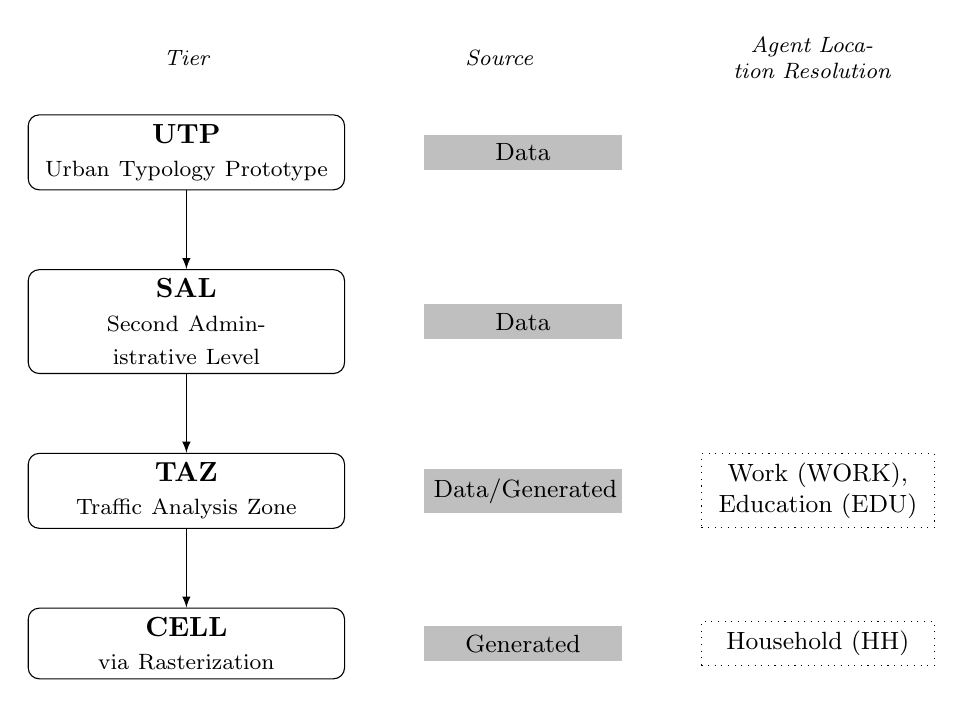
\begin{tikzpicture}[>=latex]
    \tikzset{tier/.style= {draw, rectangle, rounded corners, text width=25ex, align=center} }
    \tikzset{source/.style= {fill=gray!50!, rectangle,text width=15ex,font={\small}} }
    \tikzset{loca/.style= {draw,dotted, rectangle,text width=18ex,font={\small}} }
    \tikzset{head/.style= {draw=none,text width=18ex,font={\footnotesize\it}},align=center }
      
    \node[tier] (cell) at (0,0) {{\bf CELL}\\{\footnotesize via Rasterization}} ;
    \node[tier] (taz) [above= of cell] {{\bf TAZ}\\{\footnotesize Traffic Analysis Zone} } ;
    \node[tier] (sal) [above= of taz] {{\bf SAL} \\{\footnotesize Second Administrative Level}} ;
    \node[tier] (utp) [above= of sal] {{\bf UTP} \\{\footnotesize Urban Typology Prototype}} ;

    \node[head] (tier) [above= .5cm of utp] {Tier};
    \node[head] (source) [right= 1cm of tier] {Source};
    \node[head] (location) [right= 1cm of source] {Agent Location Resolution};
    
    \path[draw, ->] (utp) -- (sal);
    \path[draw, ->] (sal) -- (taz);
    \path[draw, ->] (taz) -- (cell);

    
    \node[source] (utp-source) [right= of utp] {Data};
    \node[source] (sal-source) [right= of sal] {Data};
    \node[source] (taz-source) [right= of taz] {Data/Generated};
    \node[source] (cell-source)[right= of cell]{Generated};

    \node[] (utp-location) [right= of utp-source] {};
    \node[] (sal-location) [right= of sal-source] {};
    \node[loca] (taz-location) [right= of taz-source] {Work (WORK), Education (EDU)};
    \node[loca] (cell-location)[right= of cell-source]{Household (HH)};
  \end{tikzpicture}
  \caption{The four tiers of the prototype city development framework. The UTP represents the urban typology, and is given by the metro area of the candidate city chosen for the supply.
  The Second Administrative Levels are the highest-level regions into which the UTP is subdivided. TAZ's are obtained for the UTP given the candidate road network. Where unavailable, these are generated as Thiessen polygons. CELLs are obtained by gridding over the SALs (or TAZs). The corresponding land use weight at the CELL level is used to determine the  {\it number} and {\it location} of the households therein; as well as the {\it numbers} of WORK and EDU points in each TAZ.}
  \label{fig:framework}
\end{figure}



\begin{table}[h!]
  \centering
  \begin{tabular}{l l l}
    &&
  \end{tabular}
  \caption{List of symbols for variables and parameters}
  \label{tab:symbols}
\end{table}





% \begin{enumerate}[Step 1:]
% \item Network: modify OSM network file, make it legal input to SimMobility
%   \begin{enumerate}[1.]
%   \item links has to be unidirectional
%   \item shorten the links and add turning points
%   \item maintain the attributes of each object in the network
%   \end{enumerate}
% \item Population Synthesis
%   \begin{enumerate}[1.]
%   \item Data collection: sample data, aggregate data for zones in each city
%   \item Data processing: categorize sample data and get joint distribution, formatting aggregate data
%   \item Apply IPF algorithm and use the weights result to draw synthetic population
%   \item Assign households in each county to locations based on land use information
%   \end{enumerate} 
% \end{enumerate}

In summary, the following are steps involving in generating a synthetic population and preparing it for mesoscopic simulation.
\begin{itemize}
\item 
\item 
\end{itemize}

\subsection{Supply}
The supply pipeline can be summarized in the following steps:
\begin{itemize}
\item Obtain candidate city for urban typology based on that closest to centroid of supply factors
\item Process road network from supply candidate and generate SimMobility inputs
\item Generate public transit graph from GTFS and other sources
\item Process land-use data polygons
\end{itemize}

\subsection{Demand}



\subsection{Geolocation and spatial assignment}
Our implementation is outlined in the following subsections.


\subsubsection{Households}
\begin{itemize}
  \item Aggregate land use categories into these: low residential ($L$), high residential ($H$), commercial ($C$), industrial ($I$), education ($E$), open land ($O$)
  \item Assign weights for households as follows:
    \begin{equation}
     HH (w_L, w_H, w_C, w_I, w_E, w_O) = (8, 10, 4, 1, 0, 0)
    \end{equation}
  \item Grid the map and assign weights to the cell $w_c^{HH}$ given its  prevailing land use category
  \item Normalize cell weights $p_{c(SAL)}^{HH}$ in each second administrative level ($SAL$)
    \begin{equation}
      p_{c(SAL)}^{HH} = \fr{w_c^{HH}}{\sum_{c \in SAL} w_c^{HH}}
    \end{equation}
  \item Number of households in each cell given by:
    \begin{equation}
     N_{HH}^{c(SAL)} = p_c^{SAL}\cdot N_{HH}^{SAL}
    \end{equation}
    where $ N_{HH}^{SAL}$ is the number of households in each $SAL$.
  \item Randomly sample to locate households in cell centroids for all $SAL$
  \end{itemize}


\subsubsection{Firms and education zones}
\begin{itemize}
  \item We obtain numbers of firms and schools in each $SAL$
  \item Assign weights as follows:
    \begin{align}
      WORK (w_L, w_H, w_C, w_I, w_E, w_O) &= (1, 2, 10, 5, 3, 1)\\
      EDU (w_L, w_H, w_C, w_I, w_E, w_O) &= (0, 0, 0, 0, 1, 0)
    \end{align}
  \item Assign weights to cells for work and education: $w_c^{WORK}$,  $w_c^{EDU}$
    
  \item Find $p_{c(SAL)}^{WORK}$ and $p_{c(SAL)}^{EDU}$ as before
  \item Find  $N_{WORK}^{c(SAL)}$ and $ N_{EDU}^{c(SAL)}$ as before
  \item The final outputs here are the numbers of workplaces/schools in each TAZ:
    \begin{align}
      N_{WORK}^{TAZ(SAL)} &= \sum_{c(SAL) \in TAZ(SAL)} N_{WORK}^{c(SAL)} \\
      N_{EDU}^{TAZ(SAL)} &= \sum_{c(SAL) \in TAZ(SAL)} N_{EDU}^{c(SAL)}  
    \end{align}
  \end{itemize}


\subsection{Trip generation and population assigment}
In this step, we estimate the number of home-based work trips and home-based education trips between zones in order to have a starting point from which to assign individuals to usual work and education zones.
The result is an OD matrix of trips from TAZ to TAZ.
From this, we then randomly assign each individual to a zone for work or education.

\subsubsection{Trip distribution}
The method for trip distribution is an entropy maximization model (analogous to the gravity model when there are no quadratic costs).

\begin{align}
  \max & - \sum_{i=1}^K\sum_{j=1}^L x_{ij} \ln x_{ij}\\
  \text{s.t.} & \sum_{j=1}^{L}x_{ij} = O_i, \quad i = 1,2, \dots,K\\
       & \sum_{i=1}^{K}x_{ij} = D_j, \quad i = 1,2, \dots,L\\
       &  \sum_{i=1}^K\sum_{j=1} c_{ij}x_{ij} = C \\
      % &  \sum_{i=1}^K\sum_{j=1} c_{ij}x_{ij} = C \\
       & x_{ij} \ge 0, \quad i =1,2,\dots,K,\; j  =1,2,\dots,L
\end{align}

The reader is referred to \citet{fang1995linearly} for a more formal background of this problem.
A fuzzy extension that accounts for uncertainty in cost estimates has also been proposed by \citet{li2011entropy}.
For now, however, we use the simple gravity approach outlined above.
A quadratic cost constraint may also be introduced later:
\begin{equation}
   \sum_{i=1}^K\sum_{j=1} d_{ij}x_{ij}^2 = D \\
\end{equation}



\subsubsection{Route assignment}
We also solve a static traffic assignment problem in order to find congested zone-zone travel times.
The input network is a graph in which the nodes are TAZes and the edges are generalized between each zone.
An average link capacity is obtained from the limiting capacity of the union of shortest paths between the zones.
The problem is a user-optimum (Wardorp) equilibrium, formulated as follows:

\begin{align}
  \min & \sum_{e_{OD} \in E} \int_{0}^{f_{OD}}tt^{OD}(x) dx \\ \notag
  \text{s.t.} & \\
  f_{OD} &= \sum_{i}\sum_{j}\sum_{r}\alpha_{ij}^{e_{OD}r}x_{ij}^{r}\\
  \sum_r x_{ij}^{r} &= x_{ij} \\
  f_{OD} &\ge 0 \\
  x_{ij}^{r}& \ge 0 \\
  \alpha_{ij}^{e_{OD}r} &=
                          \begin{cases}
                            1 & e_{OD} \in r \\
                            0 & \text{otherwise}
                          \end{cases}
\end{align}

The solution to this problem provides the equilbrium OD flows between the TAZes.
We can therefore compute congestion travel times.
The congested travel time estimates for each TAZ OD is given by
\begin{equation}
  \label{eq:tt}
  tt^{OD}(f_{OD}) = tt_0^{OD}\lt(1 + 0.15\lt( \fr{f_{OD}}{Cap_{OD}}\rt)^4\rt)
\end{equation}
where $tt_0^{OD}$ is the free-flow travel time for a given OD. 
This is the standard Bureau of Public Roads congestion function \citep{mtoi2014calibration}, which we consider sufficient for the purposes of estimating congested travel times.


\subsection{Zonal-level  estimation}
\subsubsection{Estimation of origin-destination matrices}
There are three key inputs at the zonal level required for running SimMobility preday: zonal attribute data, skim matrices, and zone-zone travel time data.


\begin{table}[h!]\small
  \centering
  \begin{tabular}{l l l } \toprule
    \textbf{Parameters}            & \textbf{Description}  & \textbf{Notes} \\ \midrule
    \texttt{distance}     & Zone-zone distance (km) & \\
    \texttt{car\_cost\_erp} & Road pricing cost (monetary units) &  \\
    \texttt{car\_ivt}     & Car in-vehicle time  (hours) & \\
    \texttt{pub\_ivt}     & Public transit in-vehicle time (hours) & \\
    \texttt{pub\_walkt}   & Public transit access-egress walking time (hours) & \\
    \texttt{pub\_wtt}     & Public transit waiting time (hours) & \\
    \texttt{pub\_cost}    & Public transit cost between zones (monetary units) & \\
    \texttt{avg\_transfer}& Average number of public transit transfers between zones & \\
    \texttt{pub\_out}     & Public transit out-of-vehicle travel time (hours) & Sum  \texttt{pub\_walkt} and  \texttt{pub\_wtt} \\ \bottomrule
  \end{tabular}
  \caption{Operating cost parameters (Skim matrix elements) in SimMobility}
  \label{tab:opcosts}
\end{table}

\subsubsection{Initial estimates}
\begin{enumerate}
\item The zone-zone distance can be readily estimated by averaging the shortest-path distances for all unique OD pairings within a pair of zones. Given $P_{n_O n_D}$ as the shortest path for a given node-node OD pair, $n_On_D$, between two zones $O$ and $D$, then we can write
  \begin{equation}
    d_{OD} = \frac{\sum_{n_On_D \in V(O) \times V(D)}|| P_{n_On_D}||}{|V(O) \times V(D)|}
  \end{equation}
\item The road pricing cost can be zero for now, but these will be relevant for congestion pricing scenarios. Thus,
  \begin{equation}
    C^{rp}_{OD} = 0
  \end{equation}
\item Car in-vehicle time $CIVT$ can be computed using free-flow speeds $FFS_e$ along each edge $e$ of the shortest-path ODs for each zone pair to travel times, which are then averaged to obtain the final estimate:
  \begin{align}
    CIVT(P) &= \sum_{e \in P} \fr{||e||}{FFS_e}\\
    CIVT_{OD} &= \frac{\sum_{n_On_D \in V(O) \times V(D)} CIVT(P_{n_On_D})}{|V(O) \times V(D)|}
  \end{align}
\item Public transit in-vehicle time $PIVT$ is estimated using the procedure outlined in (iii) applied to the public transit graph
\item Public transit access-egress times are obtained by averaging the shortest edges connecting each road node to a public transit node in zone $O$ and adding this to the corresponding value for zone $D$. We assume a walking speed of 5 km/h, and dividing the sum obtained by this value produces an estimate of the walking time for each zone $OD$ pair.

\item To estimate the public transit waiting time, we consider the median headway of the train/bus route on the first edge of all the shortest paths connecting public transit nodes in each zone-zone pairing. If there is a transfer on a given path, then the headway of the train/bus on the edge incident on the transfer point is added to the headway for the beginning of that path.

\item The public transit cost between zone $OD$s is taken as the average fare scaled by the relative average length of the shortest paths between the nodes in a given pair of zones.

\item We can compute the average number of transfers for each zone $OD$ by summing the number of transfers for the shortest paths in all node-node pairs between zones and dividing by the number of node-node pairings.
\end{enumerate}


We assume morning peak period as 7-9am and evening peak period as 5-7 pm.


\subsection{Calibration and validation}
Initially tune parameters. 
  
\subsubsection{Trip structure}
Aggregate modeshares for the typology
  
\subsubsection{Activity structure}
Consider cities near supply-demand interaction centroid:
\begin{itemize}
\item Supply-demand interaction defined by factors, namely: congestion/highway domination and inefficiency
\item If travel surveys are available: validate against activity shares
\end{itemize}


\subsection{Summary of framework}
In our first exploration, we have used 5 attributes to describe a households and they are household type, household size, household income in the last 12 months, number of vehicles and number of workers in the household. We not only find one dimensional marginal distribution for those variables but also two dimensional marginal distributions for household type $\times$ household size, number of workers $\times$ household size as well as number of vehicles $\times$ number of workers in the household. Across the process of data retrieving and processing, we find the categories each variable can have is largely depends on the availability and format of aggregate data.




\section{Results and discussion}




\section{Conclusion}
\section{References}
\printbibliography

\appendix
\section{Further notes on hierarchical iterative proportional fitting}
Using IPF to synthesize population includes two major steps.
In the first step, the disaggregate samples of population are used to initialize the contingency table expanded by attributes, and the fitting is carried out to meet marginal constraints from aggregated data.
In the next step, the fitted contingency table is used to sample the population.
To describe IPF, we need to define the contingency table it fits.
Suppose a person or household is described by \textit{m} attributes (or demographics), then we need to develop a m-way table.
For each demographic $i$, there are $n_i$ categories.
Thus, a cell $(i_1, i_2,..., i_m)$ represents a kind of person/household, where $i_j = 1,2,...n_j$ is the observed value of the $j$-th demographic with $n_j$ categories it can choose from.
From sample data like PUMS, $n$ is the total number of observations while $n_{i_1, i_2,...,i_m}$ is the counts for people/household of this type.
Hence, the proportion of this type in the sample is denoted by
\begin{equation}
  \label{eqn:prop}
   p_{i_1,i_2,...,i_m} = \frac{n_{i_1, i_2,...,i_m}}{n}
\end{equation}
The constraints is defined as $T_k^j$, which is the marginal totals for the $k$-th category of attribute $i$ from census data.
We can easily get the equation
\begin{equation}
  \label{eq:2}
\sum_i\sum_{k=1}^{n_i}T_k^j=n.  
\end{equation}
Let $p_{i_1,i_2,...,i_m}^{(t)}$ denote estimated proportion of cell $(i_1, i_2,..., i_m)$ in iteration $t$ and
\begin{equation}
  \label{eq:3}
  p_{...,i_j=k,...} = \sum_{i_1=1}^{n_1}...\sum_{i_m=1}^{n_m}p_{i_1,i_2,...,i_j=k,...,i_m}^{(t)}  
\end{equation}

The IPF starts with initiating all weights in the contingency table by  
\begin{equation}
	p_{i_1,i_2,...,i_m}^{(0)} = p_{i_1,i_2,...,i_m}
\end{equation}
and in each iteration, the proportions are updated by the formula
\begin{equation}
  p_{i_1,i_2,...,i_j=k,...,i_m}^{(new)} = p_{i_1,i_2,...,i_j=k,...,i_m}^{(old)} * \frac{T_k^j * p_{...,i_j=k,...}^{(new)}}{n} 
\end{equation} for all categories of each attribute, until it converges.
Within an iteration, $p^{(old)}$ for the first marginal corresponds to $p^{(t-1)}$, which is the result from last iteration.
And for marginals come next, $p^{(old)}$ should be set to proportions calculated from previous marginals.
According to \cite{beckman1996creating}, the algorithm converges in 10 to 20 iterations.

In the next step, the synthetic population shall be constructed by selecting households from PUMS in proportion to the estimated weights in the multiway table. Or we can do Monte Carlo sampling method to draw households from estimated weights from IPF.
Specifically, the number of households of each demographic type in a census tract can be obtained by multiplying the total number of households by the probability in the cell representing this household type, or by drawing the numbers at random according to these probabilities.
However, the household type represent by a cell in multiway table is not exactly that of PUMS data.
The fitted multiway table can only be span by control variables, which is defined as variables which have marginal distribution in census data.
However, households and individuals in disaggregate data are usually described by additional desired variables.
So, the probability of a household type in PUMS data being chosen shall be assigned according to the distance between such a household $p$ and a household type $c$ in multi-way table.
In \cite{beckman1996creating}, this probability is defined as 
\begin{equation}
  D(p,c) = w_p \prod_{i \in J}\Big(1-|(d_i^p-d_i^c)/r_i|^k\Big)*\prod_{i \notin J}\Big(1-\Delta(d_i^p, d_i^c)\Big)
\end{equation}
      
\end{document}
